\section{\color{blue} Models of quantum algorithms in sets and relations}

In this section we construct abstract models of blackbox quantum algorithms using a model of quantum computation in sets and relations, a setting that is usually considered as a model for nondeterministic classical computation.  This work provides an alternative model of quantum computation (QCRel) that, though unphysical, nevertheless faithfully models its computational structure.  Our main results are models of the Deutsch-Jozsa, single-shot Grovers, and GroupHomID algorithms in QCRel. These models provide new tools to analyze the semantics of quantum computation and improve our understanding of the relationship between computational speedups and the structure of physical theories. They also exemplify a method of extending physical/computational intuition into new mathematical settings.

\suubsection{Introduction}

Having grasped the abstract structure at play in the protocols and algorithms of quantum computation, we can conceive of modelling quantum computation in settings other than Hilbert spaces and linear maps.  There are two main thrusts that make this investigation, the subject of this paper, interesting.  The first is to further analyze the structure of quantum computation, advancing our understanding of the relationship between computational speedups and the structure of physical theories. We use the QCRel model defined here to model some example quantum algorithms as non-deterministic classical algorithms while preserving their query-complexity (and, in fact, all their abstract structure). The second thrust is for the insights that become available by extending physical/computational intuition into new areas of mathematics. While other toy models of a relational flavor for quantum mechanics have been proposed \cite{ellermanModelQM}\cite{discreteQT}\cite{modalQT}\cite{spekk}, and some even discuss protocols \cite{QCFF_James}, these works have not developed the structures necessary to model quantum algorithms.

The next section of this paper will construct our chosen model of quantum information.  This is the setting of sets and relations, rather than Hilbert spaces and linear maps, and it will be introduced by rephrasing the axioms of quantum mechanics. Section 3 will introduce a graphical notation for analyzing processes in this setting. Sections 4-9 present the novel contributions of this paper: relational models of unitary oracles, the Deutsch-Jozsa algorithm, the single-shot Grover's algorithm, and the group homomorphism identification algorithm.

\subsection{The model of quantum computation in relations}

We begin with definitions of the key components of quantum computation in this new setting, e.g. systems, states, bases, observables, etc.  The following definitions are motivated \todo{CHAPTER}, whose general theorems prove useful.

To avoid distracting repetition of notation, we use generic terminology to refer to the relational setting within this paper.  For example \emph{system} is intended to mean \emph{relational system}, i.e. a set.  When we wish to refer to the quantum setting we explicitly denote this e.g. \emph{quantum system} refers to a finite dimensional Hilbert space.

\begin{axiom}
A \emph{system} is a set $H$ with \emph{states} $|\psi\rangle$ given by subsets $\psi\subseteq H$.
\end{axiom}


\noindent Our notation is to write the set label as a ket. Thus $|\psi\vee\phi\rangle$ denotes the state with elements in the union of sets $\psi$ and $\phi$. We often use $\ket{\psi}$ to mean the relation $\{\bullet\}\to H$ that relates the singleton to all the elements in $\psi$.

\begin{axiom}
A \emph{composite system} $H$ of $n$ systems $H_1,...,H_n$ is given by the Cartesian product of the subsystem sets so that $H = H_1\times...\times H_n$. \emph{Composite states} will be written as $|\psi\times\phi\rangle$ and are any subset of the product set $H$.
\end{axiom}

\begin{defn}
For relation $R:A\to B$ from set $A$ to $B$, the \emph{converse relation} is denoted $R^{-1}:B\to A$ where for $x\in A$ and $y\in B$, $xRy$ if and only if $yR^{-1}x$.
\end{defn}

\begin{defn}
A relation $R:H_1\to H_2$ is \emph{unitary} if and only if $R\circ R^{-1} = \mbox{id}_{H_1}$ and $R^{-1}\circ R = \mbox{id}_{H_2}$, where $\circ$ is the usual composition of relations.
\end{defn}

\begin{corollary}[\cite{cqm-notes}]
\label{cor:bijections}
Relations are unitary if and only if they are bijections.
\end{corollary}

\begin{axiom}
\emph{Evolution} of systems is given by unitary relations.
\end{axiom}

\noindent This means that states of system $A$ can evolve to a state of system $B$ if and only if there is a bijection between them. Note that this implies that there do not exist physical evolutions between systems of different cardinality. 
%This is analogous to the quantum setting where there do not exist unitary %maps between Hilbert spaces of differing dimensions.

\begin{defn}
For a state $\ket{\psi}:\{\bullet\}\to H$, denote its relational converse as $\bra{\psi}:H\to\{\bullet\}$ called its \emph{effect}.
\end{defn}

\noindent A state preparation followed by an effect amounts to an experiment with a post-selected outcome. Effects are maps to $\{\bullet\}$ that return if the outcome state $\ket{\psi}$ is possible.
 We give an example to illustrate:
\begin{example}
The preparation of the state $\ket{\phi}$ followed by a post-selected measurement of the effect $\bra{\psi}$ is given by the relation
\begin{align*}
\langle\psi|\phi\rangle:=\bra{\psi}\circ\ket{\phi}:\{\bullet\}\to H\to \{\bullet\}
\end{align*}
This is either the identity relation that we interpret to mean a measurement of $\ket{\psi}$ is \emph{possible}, or it is the empty relation that we interpret to mean the measurement outcome $\ket{\psi}$ is \emph{impossible}. It is clear that the outcome $\ket{\psi}$ is possible if there exists some element of $H$ in both $\psi$ and $\phi$. Otherwise it is impossible.
In this sense our relational quantum computation is a deterministic model of quantum computation.
\end{example}

This interpretation allows us to define a generalized version of the Born rule to describe measurement in our model.
\begin{axiom}[Generalized Born Rule]
The possibility of measuring the state $\ket{\psi}$, having prepared state $\ket{\phi}$, is given by the image of:
\begin{align}
\langle\psi|\phi\rangle:\{\bullet\}\to\{\bullet\}
\end{align}
\end{axiom}

In the relational model, bases are characterized as particular generalizations of groups known as \textit{groupoids} \cite{pavlovic-2009}\cite{evans2009classifying}.  Groupoids can be viewed as groups where multiplication is relaxed to be a partial function.

\begin{defn}
\label{def:basis}
For a system $H$, a \emph{basis} $Z$ is list of abelian groups $Z = G_0\oplus G_1\oplus...$ where $\sum_G |G| = |H|$.
Multiplication with respect to this list of groups will be written as $\bullet_Z$ and is defined in the following way. For elements $x,y\in Z$ such that $x\in G_i$ and $y\in G_j$ we have the partial function:
\begin{align}
\label{eq:groupoid_mult}
x\bullet_Zy = \begin{cases}i=j & x +_{G_i} y \\
\mbox{otherwise} & \mbox{undefined}\\
\end{cases}
\end{align}
\noindent This makes $Z$ an \emph{abelian groupoid} with groupoid multiplication $\bullet_Z$.
\end{defn}

At first guess, one might be motivated by the intuition that a basis for a system breaks it up into parts, and so a basis would be a partition of $H$.  This is not a bad start, however, basis have additional structure: namely that we can copy, delete and combine them at will.  This idea is used to motivate Definition \ref{def:basis} by abstracting bases to classical structures. \todo{REF APPROPRIATE DEFINITIONS}.
Their classical-like properties, allowing copying, deleting, and combining, give them this name. The definition of a special dagger-commutative Frobenius algebra in our model is given in Section \ref{section:graphical}, but we can interpret it through pair of lemmas corresponding to the traditional-model and the relational-model of quantum computation.
\begin{lemma}[\todo{reference from other section}]
\label{lem:sdfa-hilb}
Classical structures in the category of finite dimensional Hilbert spaces and linear maps are exactly orthogonal bases.
\end{lemma}

\begin{lemma}[\cite{evans2009classifying}]
\label{lem:sdfa-rel}
Classical structures in the category of sets and relations are exactly abelian groupoids.\footnote{In \cite{heunen-relFrob} this connection is extended to the non-abelian case where it is shown that all relative Frobenius algebras as groupoids.}
\end{lemma}

\subsubsection*{Complementarity}
Complementary bases\footnote{Theorem \ref{thm:compl} holds as long as we consider bases to be the same if their lists of groups are isomorphic.} in the relational setting are understood using a different abstraction that more narrowly specifies their structure:
\begin{theorem}[\cite{cqm-notes}\todo{better reference}]
\label{thm:compl}
Two bases $Z$ and $X$ are complementary if and only if they are of the following form. Basis $Z = \bigoplus^{|H|}G$ and basis $X = \bigoplus^{|G|}H$ given by copies of abelian groups $G$ and $H$ respectively.
\end{theorem}

This theorem follows from the requirement that the classical points of one observable must be isomorphic to the unbiased points of its complement. We will return to this idea in the Section \ref{sec:FT} when we address the quantum Fourier transform.

Classical and unbiased points of bases in the relational model are specified in the following corollaries. An example on the six element system is illustrated with Figure \ref{complEx}.

\begin{figure}[tb]
\begin{center}
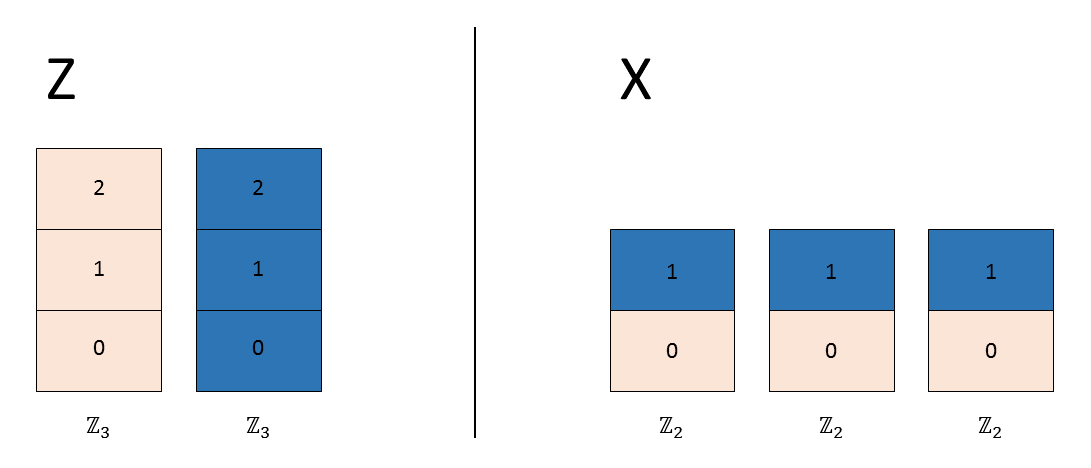
\includegraphics[height=14em,natwidth=1091,natheight=468,scale=1]{images/complexample.png}
\end{center}
\caption{An example of two complementary bases on the system of six elements. Here $Z=\mathbb{Z}_3\oplus\mathbb{Z}_3$ and $X = \mathbb{Z}_2\oplus\mathbb{Z}_2\oplus \mathbb{Z}_2$.  The two classical points of $Z$ are each three element subsets and are colored in pink and blue. The unbiased points of $X$ to which they correspond are colored to match.
}
\label{complEx}
\end{figure}

\begin{corollary}
The \emph{classical points} of a basis $Z$ are the subsets of $H$ corresponding to the groups $G_0, G_1,...$ where we forget the group structure. They will often be denoted $\ket{G_i}$.
\end{corollary}

\begin{corollary}
The \emph{unbiased points} for a basis $Z$ on a system $H$ are subsets $U\subseteq H$ such that for a fixed $g\in G$,
\begin{align*}
\ket{U} = \bigcup_{h\in H}g .
\end{align*}
Thus there is exactly one element in $U$ from each component $G_i$ of $Z$.
\end{corollary}

\begin{example}
Take $Z = \mathbb{Z}_2\oplus\mathbb{Z}_2=\{0_a,1_a,0_b,1_b\}$. The classical points of $Z$ are $\ket{G_0}=\ket{0_a\vee1_a}$ and $\ket{G_1}=\ket{0_b\vee1_b}$.  The unbiased points of $Z$ are $\ket{U_0}=\ket{0_a\vee0_b}$ and $\ket{U_1}=\ket{1_a\vee1_b}$.
\end{example}

It is easy to check that complementary observables as specified by Theorem \ref{thm:compl} have the property that each classical point $\ket{G_i}$ of the observable $Z$ corresponds to one unbiased point of $X$ and vice versa, i.e. $\ket{U_i}=\ket{H_i}$.

\subsubsection*{Phases}

Phases are also defined in this relational setting.  In Hilbert space quantum mechanics a quantum phase for an n-dimensional system is given by the vector
\begin{align*}
\left(\begin{array}{c}
e^{i\phi_1} \\
\vdots \\
e^{i\phi_n}
\end{array}
\right).
\end{align*}
These quantum phases form an abelian group and can be applied as phase gates.
Their relational counterparts are described by the following lemma from \cite{cqm-notes}:
\begin{lemma}
For a basis $Z=\bigoplus_i^NG_i$, the \emph{phase group} $B(Z)$ is given by $\prod_i^NG_i$.
\end{lemma}

\begin{example}
Consider the basis $\mathbb{Z}_2\oplus\mathbb{Z}_2$ for the four element system $\{00,01,10,11\}$.  Let $|\psi\rangle$ be the state $|00\vee10\rangle$. Application of the phase $11$ results in
\[ 11|00\vee10\rangle = |11\vee01\rangle . \]
\end{example}

We are also able to interpret GHZ states and density matrices in sets and relations.

\begin{defn}
For a basis $Z$, a \emph{GHZ} state is given by
\[ GHZ_Z \; := \{\;(a,b,c)\;|\;\ \forall \;a,b,c \in Z,\;a\bullet_Zb\bullet_Zc = \mbox{id}_{G_i}\mbox{ for some } i\;\}.  \]
\end{defn}

\begin{defn}
For a state $|\psi\rangle$, the \emph{density matrix} $|\psi\rangle\langle\psi|$ is given by the relation $xRy$ s.t. $x,y\in \psi$.
\end{defn}

\subsubsection*{The model QCRel}

\begin{defn}
Axioms 1-4, and subsequent definitions, specify the abstract process theory for \emph{quantum computation in relations}: QCRel.
\end{defn}

\begin{theorem}
QCRel is a model of quantum computation with sets and unitary relations.
\end{theorem}
\begin{proof}
This is true by construction.  The axioms on the preceding section can be interpreted as structures in any dagger compact category. In particular, {\bf FHilb}, the category of finite dimensional Hilbert spaces and linear maps,  is a dagger compact category in which interpretation of those axioms results in the usual Hilbert space quantum mechanics.

{\bf Rel}, the category of sets and relations, is also dagger compact.  It is the interpretation of the abstract axioms for quantum computation in {\bf Rel}, rather than {\bf FHilb}, that produces QCRel as a model. A reference that covers the dagger compact abstraction and some of its interpretation in different categories is \cite{cqm-notes}.
\end{proof}

It is worth noting that QCRel can be simply viewed as a local hidden variable theory. We consider the set $H$ to be the set of ontic states such that for $\phi\subseteq H$ the state $\ket{\phi}$ is non-deterministically in any of the ontic states in the subset $\phi$.  From this perspective, QCRel provides a non-deterministic local hidden variable model for computational aspects of quantum mechanics.\footnote{See \cite{abramsky2012operational} for details of this interpretation as an operational theory.}  This means that protocols exist for entanglement, teleportation, and, as we show in this paper, some familiar blackbox algorithms.

\subsubsection*{Unitary Oracles}

In order to model blackbox quantum algorithms in this setting, we must define the oracles themselves.
We do this by building up from an abstract definition of the controlled-not gate from the literature. Let the gray classical structure on a system $A$ be given by a basis $Z=\bigoplus^{|H|}G$ and the white classical structure be a basis $X=\bigoplus^{|G|}H$. The comonoid for the gray dot is then the relation $\tinycomult[graydot]:A\to A\times A$ that for $x,a,b\in H$ given by
\[ \{(x,(a,b))~|~a\bullet_Zb=x\}. \]

\begin{defn}[\cite{zeng-unitary}\todo{ref back}]
\label{eq:generalizedcnot}
The abstract controlled-not is given by a composition of the comonoid for Z and the monoid for X:
\begin{equation*}
\,\,
\begin{aligned}
\begin{tikzpicture}[xscale=\tikzxscale, yscale=\tikzyscale]
\node (b) [graydot] at (0,0) {};
\node (w) [whitedot] at (1,1) {};
\draw (-0.75,2) to [out=down, in=left] (b.center);
\draw (b.center) to [out=right, in=left] (w.center);
\draw (w.center) to (1,2);
\draw (b.center) to (0,-1);
\draw (w.center) to [out=right, in=up] (1.75,-1);
\end{tikzpicture}
\end{aligned}
\end{equation*}
whose explicit relation is:
\begin{align}
\label{eq:cnot_rel}
\mbox{CNOT}:H\times H\to H\times H :: \{((x,y),(a,b\circ_Xy))~|~a\bullet_Zb=x\}.
\end{align}
\end{defn}
It can be shown that in the traditional quantum setting of Hilbert spaces and linear maps, this exactly corresponds to the usual controlled-not. This also leads to the following useful theorem, which can be abstractly proved.

\begin{theorem}[Complementarity via a unitary \cite{zeng-unitary}\todo{ref back}]
\label{thm:complementarityunitary}
  Two symmetric dagger-Frobenius algebras are complementary if and only if the abstract controlled-not from Definition \ref{eq:generalizedcnot} is unitary.
\end{theorem}

\noindent This allows us to prove the following statement about  complementary bases in QCRel.
\begin{theorem}
Two bases in QCRel are complementary, in the sense of Theorem \ref{thm:compl}, if and only if the relation in Equation \ref{eq:cnot_rel} is a bijection.
\end{theorem}
\begin{proof}
The relevant relation can clearly be seen to be the composite in Definition \ref{eq:generalizedcnot} as
\begin{align}
\{((a,b,y),(a,b\circ_Xy))\} \circ \{((x,y),(a,b,y))~|~a\bullet_Zb=x\}.
\end{align}
Thus the abstract proof of\ Theorem \ref{thm:complementarityunitary} from \cite{zeng-unitary} goes through unchanged.
\end{proof}

An oracle is then introduced as a controlled-not where we have embedded a particular kind of relation that abstractly must be a self-conjugate comonoid homomorphism \cite{zeng-unitary} \todo{ref back}. We construct such relations in the following lemmas.

\begin{defn}
Given groupoids $G$ and $H$ and groupoid homomorphism $F:G\to H$, we can define an associated \emph{groupoid homomorphism relation} $R:G\to H$ where, for morphism $x$ in $G$ and morphism $y$ in $H$,
$$
xRy \mbox{ iff }F(x) = y.
$$
\end{defn}

\begin{lemma}
\label{lem:mongrphom}
Given a groupoid homomorphism that is surjective on objects, its associated groupoid homomorphism relation $R:G\to H$, is a monoid homomorphism relation.
\end{lemma}
\begin{proof}
A groupoid homomorphism $F:G\to H$ is a functor that, for objects $X,A,B$ of $G$ and morphisms $f$ of $G$, takes
\begin{align*}
X &\mapsto F(X) \\
(f:A\to B) &\mapsto \left(F(f):F(A)\to F(B)\right)
\end{align*}
such that
\begin{align*}
F(g\circ_G f) &= F(g)\circ_H F(f) \\
F(\mbox{id}_X) &= \mbox{id}_{F(X)}.
\end{align*}
We now show that the groupoid homomorphism relation $R$ associated to $F$ is a monoid homomorphism relation.

First, we must show that it preserves the unit, i.e. that for $X\in\mbox{Ob}(G)$  and $Y\in\mbox{Ob}(H)$ we have $R(\bigcup_X \mbox{id}_X) = \bigcup_Y \mbox{id}_Y$. Recall that for a set $A$ with elements $a$, $R(A)=\bigcup R(a)$. It is that case that
\begin{align}
R(\bigcup_X \mbox{id}_X) &= \bigcup_XR(\mbox{id}_X) \\
&= \bigcup_X\mbox{id}_{R(X)} \qquad \mbox{def. of functor} \\
&= \bigcup_{R(X)}\mbox{id}_{R(X)} \\
&= \bigcup_{Y}\mbox{id}_{Y} \qquad \mbox{surjective on objects}
\end{align}
where we have used the fact that $F$ is surjective on objects, which implies that every object of $H$ is in the image of $R$ and that $|\mbox{Ob}(G)|\ge|\mbox{Ob}(H)|$.

The second monoid homomorphism condition is to preserve multiplication, i.e. that for subsets $K$ and $J$ of $G$ we have
\begin{align}
R(K+_GJ)=R(K)+_HR(J).
\end{align}
Here we recall that for two sets $A$ and $B$, $A+B=\bigcup(a+b)$ for all $a\in A$ and $b\in B$. Thus,
\begin{align}
R(K+_GJ) = R(\bigcup_{k,j}k+_Gj) &= \bigcup_{k,j}R(k+_Gj) \\
&= \bigcup_{k,j}R(k)+_HR(j) \qquad \mbox{def. of functor}\\
&= R(K)+_HR(J).
\end{align}
This completes the proof.
\end{proof}

In fact, when the monoid is part of a classical structure (and so given by groupoid multiplication) is it easy to see that all the monoid homomorphism relations come in the form of Lemma \ref{lem:mongrphom}.

We then dualize the proof of Lemma \ref{lem:mongrphom} to conclude that:
\begin{lemma}
\label{lem:classicalRelation}
For a functor $F:H\to G$ such that $F^{\mbox{\tiny op}}$ is a groupoid homomorphism that is surjective on objects, $F$ defines a comonoid homomorphism relation.
\end{lemma}
\noindent We call these comonoid homomorphism relations \emph{classical relations}. These are relations that properly preserve the structure of the bases where classical data is embedded.  In the quantum case they take basis elements to basis elements. Some examples\footnote{These examples were generated with Mathematica code that is available at https://github.com/willzeng/GroupoidHomRelations} in QCRel are listed in Appendix \ref{app:clRel}. In order to define unitary oracles, we will also need these relations to be self-conjugate by Definition \ref{def:selfconj}.

\begin{lemma}
All classical relations $f:Z^A\to Z^B$ between groupoids $Z^A=\bigoplus^NG^B$ and $Z^B=\bigoplus^{N'}G^B$ are self-conjugate.
\end{lemma}
\begin{proof}
In QCRel, our dagger-Frobenius structures are groupoids and, if they are complementary to some other groupoid, then they are of the form $Z^A=\bigoplus^NG$ and $Z^B=\bigoplus^{N'}H$. We annotate the definition of self-conjugacy for some arbitrary element $(g,n)$, the element $g$ from the $n$-th group:
\begin{equation}
\begin{aligned}
\begin{tikzpicture}[xscale=2*\tikzxscale, yscale=2*\tikzyscale]
\node [morphism] (f) at (2,1) {$f$};
\draw (0,-1) to [out=up, in=left, in looseness=0.9] (1,2) node [graydot] {} to (1,2.5) node [graydot] {};
\draw (1,2) to [out=right, in=up] (f.north);
\draw (f.south) to [out=down, in=left] (3,-0.7) node [blackdot] {} to [out=right, in=down, out looseness=0.9] (4,3);
\draw (3,-0.7) to (3,-1.2) node [blackdot] {};
\node [graydot] at (1,2) {};
\node at (0,-1.25) {\small $(g,n)$};
\node at (-0.25,1.5) {\small $(g,n)$};
\node at (1,3) {\small $\langle\bigcup_n(\mbox{id}_G,n)|$};
\node at (2.5,1.7) {\small $(g^{-1},n)$};
\node at (2.1,-0.15) {\small $f^{-1}(g^{-1},n)$};
\node at (4.3,0) {\small $\left[f^{-1}(g^{-1},n)\right]^{-1}$};
\node at (3,-1.7) {\small $\langle\bigcup_{n'}(\mbox{id}_H,n')|$};
\end{tikzpicture}
\end{aligned}
\quad=\quad
\begin{aligned}
\begin{tikzpicture}[string]
\node (f) at (0,0) [morphism] {$f^{-1}$};
\draw (0,-1.5) to (f.south);
\draw (f.north) to (0,1.5);
\node at (0,-2) {\small $(g,n)$};
\node at (0,2) {\small $f^{-1}(g,n)$};
\end{tikzpicture}
\end{aligned}
\end{equation}
Thus, a relation is self-conjugate if and only if for all elements $(g,n)$ it is the case that $[f^{-1}(g^{-1},n)]^{-1}=f^{-1}(g,n)$. From Lemma \ref{lem:classicalRelation} the inverse of the classical relation $f$ is a groupoid homomorphism, so this condition will hold.
\end{proof}

Classical relations, as self-conjugate comonoid homomorphisms, will allow us to define unitary oracles.

\begin{defn}[Oracle\cite{zeng-unitary} \todo{ref back}]
\label{oracle}
Given a groupoid $Z^A:\blackcomonoid{A}$, a pair of complementary groupoids $Z^B:\graycomonoid{B}$ and $X^B:\whitecomonoid{B}$, and a classical relation $R : \blackcomonoid{A} \to \graycomonoid{B}$, an \emph{oracle} is defined to be the following endomorphism of $A \times B$:
\begin{equation}
\label{eq:reloracle}
\begin{aligned}
\begin{tikzpicture}[xscale=2*\tikzxscale, yscale=2*\tikzyscale]
    \node (dot) [blackdot] at (0,1) {};
    \node (f) [morphism] at (0.7,2) {$R$};
    \node (m) [whitedot] at (1.4,3) {};
\draw (0,0.25)
        node [below] {$A$}
    to (0,1)
    to [out=left, in=south] (-0.7,2)
    to (-0.7,3.75)
        node [above] {$A$};
\draw (0,1)
    to [out=right, in=south] (f.south);
\draw  (f.north)
    to [out=up, in=left] (1.4,3)
    to [out=right, in=up] +(0.7,-1)
    to (2.1,0.25)
        node [below] {$B$};;
\draw (m.center) to +(0,0.75) node [above] {$B$};
\end{tikzpicture}
\end{aligned}
\end{equation}
\end{defn}

\noindent In our setting this morphism is exactly
\begin{align}
\mbox{OracleRel}:A\times B\to A\times B :: \{((x,y),(a,c\circ_Xy))~|~\exists b\in A, s.t.~a\bullet_Yb=x\mbox{ and }bRc\},
\end{align}
and we are able to recall the following theorem:
\begin{theorem}
\label{thm:familyofunitaries}
Oracles are unitary.
\end{theorem}
\begin{proof}
Proved in the abstract setting for Definition \ref{oracle} \todo{in REF\ BACK}.  In that proof, oracles are shown to be unitary when $f$ is a self-conjugate comonoid homomorphism. Any classical relation, by Lemma \ref{lem:classicalRelation}, will be a self-conjugate comonoid homomorphism. Though there are others, classical relations will be sufficient for our purposes as the algorithms that follow have the additional requirement that the comonoids be part of classical structures, in which case classical relations are the only ones.
\end{proof}

\begin{corollary}
OracleRel is a bijection.
\end{corollary}
\begin{proof}
This follows directly from Theorem \ref{thm:familyofunitaries} and Corollary \ref{cor:bijections}.
\end{proof}

\subsection{The Fourier transform in relations}
\label{sec:FT}

In these algorithms we use the relational quantum Fourier transform for relations  \todo{from section TODO}. This is a generalized quantum Fourier transform whose definition is motivated as a relationship between classical and unbiased points of two observables.  For abelian groups $G$ and $H$, consider two groupoids $Z=\bigoplus^{|H|}G$ and $X=\bigoplus^{|G|}H$ to be complementary bases of the same system.

\begin{defn}
\label{def:FTRel}
The \emph{quantum Fourier transform in relations} corresponds to preparing classical points of $Z$ and measuring them against classical points of $X$.
%is an isomorphism from the classical points of $Z$ to the unbiased points %of $X$, i.e.
%\begin{align*}
%\{G_h\}\mapsto \{h_g|\forall g\in G\}
%\end{align*}
\end{defn}

\begin{example}
Take $G=\mathbb{Z}_2=\{0,1\}$, $H=\mathbb{Z}_1=\{\star\}$, $Z = G = \{ 0_\star,1_\star \}$ and $X=H\oplus H = \{ \star_0,\star_1 \}$. The computational basis is the family $\ket{H_g}_{g:G}$ of classical points for $X$, i.e. $H_0 = \{(\star,0)\}$ and $H_1 = \{(\star,1)\}$. The quantum Fourier basis is a single classical point $G_\star = \{(\star,0), (\star,1)\}$ for $Z$. In this case all states can be prepared in the computational basis, but the measurement in the quantum Fourier basis will be trivial.
\end{example}

\begin{example}
Take $G=\mathbb{Z}_2=\{0,1\}$, $H=\mathbb{Z}_2=\{a,b\}$, $Z = G \oplus G = \{ 0_a,1_a,0_b,1_b\}$ and $X= H \oplus H = \{ a_0, b_0, a_1, b_1 \}$. The computational basis is the family $\ket{H_g}_{g:G}$ of classical points for $X$, i.e. $H_0 = \{(a,0),(b,0)\}$ and $H_1 = \{(a,1),(b,1)\}$. The quantum Fourier basis is the family $\ket{G_h}_{h:H}$ of classical points for $Z$, i.e. $G_a = \{(a,0),(a,1)\}$ and $G_b = \{(b,0),(b,1)\}$.
\end{example}

See \cite{strongCompFT} to fully motivate this definition of the Fourier transform in QCRel and for its relationship to the usual Hadamard and Fourier transforms for Hilbert spaces and linear maps.

\subsection{The Deutsch-Jozsa algorithm in QCRel}

The well known Deutsch-Jozsa algorithm is an early quantum algorithm that demonstrates a speedup over exact classical computation \cite{deutsch1992rapid}. It takes as input a function promised to be either constant or balanced and returns which deterministically and with a single oracle query. In this section, we model the algorithms steps in QCRel just as it is implemented with Hilbert spaces and linear maps. This approach is somewhat dual to the usual one where different algorithms are compared on the same problem. Here we run the same abstract protocol (implemented in a different model) with the same query complexity and compare the different problems that it solves.

To run this algorithm in QCRel we use two systems.  System $A$ has cardinality $n$ and system $B$ has cardinality $\ge 2$. Take $Z^A=\bigoplus^{|H^{A}|}G^A$ and $X^A=\bigoplus^{|G^{A}|}H^A$ to be complementary bases of $A$. Take $Z^B=\bigoplus^{|H^{B}|}G^B$ and $X^B=\bigoplus^{|G^{B}|}H^B$ to be complementary bases of $B$, such that $X^B$ has at least two classical points. In analogy with the usual specification, the algorithm proceeds with the following steps.
\begin{enumerate}
\item Prepare $A$ in the zero state $|G^{A}_0\rangle$. Prepare $B$ in the state given by second classical point of $Z^B$, i.e. $|G^B_1\rangle$.

\item Apply the Fourier transform, as given by Definition \ref{def:FTRel}, to each system, resulting in states $\ket{H_0^A}$ and $\ket{H_1^B}$ respectively.

\item Apply an oracle from Equation \ref{eq:reloracle}, built from a classical relation $f:Z^A\to Z^B$.

\item Again apply the Fourier transform to system $A$ and then measure it in the $Z$ basis.
\end{enumerate}

\noindent This sequence of steps is an instance in sets and relations of the abstract Deutsch-Jozsa algorithm from \cite{vicary-tqa}, which translates to the relation:


\begin{equation}
\label{eq:reldj}
\begin{pic}[xscale=2*\tikzxscale, yscale=2*\tikzyscale]
    \node (dot) [blackdot] at (0,1) {};
    \node (f) [morphism] at (0.7,2) {$f$};
    \node (m) [whitedot] at (1.4,3) {};
\draw (0,0.25)
        node [blackdot] {}
    to (0,1)
    to [out=left, in=south] (-0.7,2)
    to (-0.7,3.75)
        node [blackdot] {};
\draw (0,1)
    to [out=right, in=south] (f.south);
\draw  (f.north)
    to [out=up, in=left] (1.4,3)
    to [out=right, in=up] +(0.7,-1)
    to (2.1,0.25)
        node [graydot] {};
\node at (2.15,0.25) [anchor=west] {$|H^B_1\rangle$};
\node at (0.05,0.25) [anchor=west] {$|H^A_0\rangle$};
\node at (-0.65,3.75) [anchor=west] {$\langle H^A_0|$};
\draw (m.center) to +(0,0.75)
        node [above] {};
\draw [thin, dashed] (-1.25,0.7) to (7.5,0.7);
\draw [thin, dashed] (-1.25,3.3) to (7.5,3.3);
\node at (4,0) [anchor=west] {Prepare initial states};
\node at (4,2) [anchor=west] {Apply a unitary map};
\node at (4,4) [anchor=west] {Measure the first system};
\end{pic}
\end{equation}

\begin{theorem}[\cite{vicary-tqa}]
\label{def:bc}
In any dagger compact category with complementary observables, the algorithm in Equation \ref{eq:reldj} will, with a single oracle query, distinguish \emph{constant} and \emph{balanced} classical relations $f:Z^A\to Z^B$ according to the following abstract definitions:
\begin{equation}
\label{eq:bc}
\mbox{\\ constant}:\quad
\begin{aligned}
\begin{tikzpicture}[xscale=2*\tikzxscale, yscale=2*\tikzyscale]
\node (f) [morphism] at (0,0) {$f$};
\draw (0,-1) to (f.south);
\draw (f.north) to (0,1);
\end{tikzpicture}
\end{aligned}
\quad=\quad
\begin{aligned}
\begin{tikzpicture}[xscale=2*\tikzxscale, yscale=2*\tikzyscale]
\draw (0,-1) to (0,-.4)
    node [blackdot] {};
\draw (0,0.5) node [state] {$x$} to (0,1);
\end{tikzpicture}
\end{aligned}
\qquad\qquad\qquad \mbox{balanced:\quad}
\begin{aligned}
\begin{tikzpicture}[xscale=2*\tikzxscale, yscale=2*\tikzyscale]
\node [morphism] (f) at (0,0) {$f$};
\draw (0,-0.85) node [blackdot] {} to (f.south);
\draw (f.north) to (0,0.75) node [graydot, hflip] {};
\node at (0.05,0.75) [anchor=west] {$2$};
\end{tikzpicture}
\end{aligned}
\quad=\quad
0,
\end{equation}
where \begin{tikzpicture}[string]
\draw (f.north) to (0,0.75) node [graydot, hflip] {};
\node at (0.05,0.75) [anchor=west] {$2$};
\end{tikzpicture} is the dagger adjoint of the second classical point of $X^B$.
\end{theorem}
That these definitions coincide with the usual ones for constant and balanced functions is shown in \cite{vicary-tqa}. In QCRel, the effect \begin{tikzpicture}[string,scale=0.75]
\draw (f.north) to (0,0.75) node [graydot, hflip] {};
\node at (0.05,0.75) [anchor=west] {$2$};
\end{tikzpicture} is $\langle H^B_1|$, which acts as a measurement of system $A$ after applying the oracle.

We illustrate the details of the QCRel model of the Deutsch-Jozsa algorithm first by example and then with general definitions.

\begin{example}
Take $A=\{0,1,2,3\}$ and $B=\{a,b,c,d\}$ to be four element systems. We define complementary observables on these systems as the following:
\begin{align*}
\begin{tabular}{|c|c|}\hline
System $A$ & System $B$ \\\hline
$Z^A = \mathbb{Z}_2\oplus\mathbb{Z}_2 \mbox{~~s.t.}$ & $Z^B = \mathbb{Z}_2\oplus\mathbb{Z}_2\mbox{~~s.t.}$ \\
$G_0^A=\{0,1\},G_1^A=\{2,3\}$ & $G_0^B=\{a,b\},G_1^B=\{c,d\}$ \\ \hline
$X^A = \mathbb{Z}_2\oplus\mathbb{Z}_2 \mbox{~~s.t.}$ & $X^B = \mathbb{Z}_2\oplus\mathbb{Z}_2\mbox{~~s.t.}$ \\
$H_0^A=\{0,2\},H_1^A=\{1,3\}$ & $H_0^B=\{a,c\},H_1^B=\{b,d\}$ \\ \hline
\end{tabular}
\end{align*}

From Equation \ref{eq:bc}, we then define constant and balanced classical relations using the following dictionary:
\begin{align}
\begin{aligned}
\begin{tikzpicture}[xscale=2*\tikzxscale, yscale=2*\tikzyscale]
\draw (0,0.2) to (0,0.75) node [blackdot, hflip] {};
\node at (0.05,0.75) [anchor=west] {};
\end{tikzpicture}
\end{aligned}
&\quad= \{(0,\bullet),(2, \bullet)\},  \quad \mbox{the adjoint of the first classical point of } X^A \\
\begin{aligned}
\begin{tikzpicture}[xscale=2*\tikzxscale, yscale=2*\tikzyscale]
\node (x) [state, xscale=0.75] at (0,0) {$x$};
\draw (0,0) to (0,0.5) {};
\end{tikzpicture}
\end{aligned}
&\quad= \{(\bullet,a),(\bullet,b)\}\mbox{ OR }\{(\bullet,c),(\bullet,d)\},  \quad \mbox{a classical point of }Z^B \\
\begin{aligned}
\begin{tikzpicture}[xscale=2*\tikzxscale, yscale=2*\tikzyscale]
\draw (0,0.2) to (0,0.75) node [graydot, hflip] {};
\node at (0.05,0.75) [anchor=west] {$2$};
\end{tikzpicture}
\end{aligned}
&\quad=\{(b,\bullet),(d, \bullet)\},  \quad \mbox{the adjoint of the second classical point of } X^B \\
\begin{aligned}
\begin{tikzpicture}[xscale=2*\tikzxscale, yscale=2*\tikzyscale]
\node (x) [blackdot] at (0,0) {};
\draw (0,0) to (0,0.5) {};
\end{tikzpicture}
\end{aligned}
&\quad= \{(\bullet,0),(\bullet,2)\},  \quad \mbox{the first classical point of } X^A
\end{align}

Thus there are two constant classical relations\footnote{A full list of classical relations is given in the Appendix.} $f:Z^A\to Z^B$, one for each classical point of $Z^B$. They are:
\begin{align}
\{ (0,a) (0,b) (2,a) (2,b) \} \quad \mbox{and} \quad
\{ (0,c) (0,d) (2,c) (2,d) \}
\end{align}
By Definition \ref{def:bc}, balanced classical relations are those which do not relate $0$ or $2$ to either $b$ or $d$. Here is the list of balanced classical relations for this example:
\begin{align*}
\{(0,c)   (2,c)   (1,d)   (3,d)\}\\
\{(2,a)   (3,b)   (0,c)   (1,d)\}\\
\{(0,a)   (1,b)   (2,c)   (3,d)\}\\
\{(0,a)   (2,a)   (1,b)   (3,b)\}
\end{align*}
For a classical relation promised to be in one of these two classes, we can distinguish which with a single oracle query.
\end{example}

We generalize these definitions of constant and balanced classical relations to the following:
\begin{definition}
\label{def:const}
A \emph{constant relation} $f:Z^{A}\to Z^{B}$ relates all elements of $A$ to a single classical point of $Z^B$.
\end{definition}

\begin{definition}
\label{def:balanced}
A relation $f:Z^{A}\to Z^{B}$ is \emph{balanced} when no element in the first classical point of $X^{A}$ is related to an element in the second classical point of $X^{B}$.
\end{definition}

\begin{theorem}
\label{thm:dj_speedup}
The Deutsch-Jozsa algorithm defined above distinguishes constant relations from balanced relations in a single oracle query.
\end{theorem}
\begin{proof}
This follows immediately from the abstract proof of the Deutsch-Jozsa algorithm in \cite{vicary-tqa}.
\end{proof}

This result shows that we are able to model the Deutsch-Jozsa algorithm in the nondeterministic classical setting of QCRel.

\subsection{Single-shot Grover's algorithm}

Grover's algorithm \cite{grover1996fast} takes as input a set $S$ and an indicator function $f:S\to\{0,1\}$. Though the algorithm is usually probabilistic and runs a repeated series of ``Grover steps", here we consider the deterministic version that runs with a single step. Our setup requires the set $S$, as one system, as well as another system $B=\{0,1\}$. We define the basis $Z^{S}=\bigoplus^NG$ and $X^S=\bigoplus^{|G|}H$ on the $S$ system.  System $B$ has complementary bases $Z^B=\mathbb{Z}_2$ and $X^B=\mathbb{Z}_1\oplus\mathbb{Z}_1$.

In QCRel, the algorithm proceeds by the following steps:
\begin{enumerate}
\item Prepare system $S$ in the state $\ket{G_0}$ and system B in the state $\ket{\sigma} = \ket{0\vee 1}$.

\item Apply the Fourier transform to system $S$, resulting in state $\ket{H_0}$.

\item Apply the oracle for a classical indicator relation $R:Z^S\to Z^B$.

\item Apply a diffusion relation $D:S\to S$ to system $S$.

\item Measure system $S$ in the $X^S$ basis.

\end{enumerate}

The diagrammatic presentation for this procedure from \cite{vicary-tqa} is:
\begin{equation}
\label{eq:grovertopological}
\begin{aligned}
\begin{tikzpicture}[xscale=2*\tikzxscale, yscale=2*\tikzyscale]
\begin{pgfonlayer}{foreground}
    \node (f) [smallbox, anchor=south, thick] at (0.7,2) {$R$};
\end{pgfonlayer}
    \node (dot) [blackdot] at (0,1) {};
    \node (m) [whitedot] at ([xshift=0.7cm, yshift=1cm] f.north) {};
\draw (0,-0.25)
        node [blackdot] (bdot) {}
    to (0,1)
    to [out=\nwangle, in=south] (-0.7,2)
    to ([yshift=1.4cm] m.center -| -0.7,1)
        node (rho) [smallbox] {$\rho$};
\draw (0,1)
    to [out=\neangle, in=south] (f.south)
    to (f.north)
    to [out=up, in=\swangle] +(0.7,1)
    to [out=\seangle, in=up] +(0.7,-1)
    to (2.1,-0.25)
        node [smallbox] (sigmadag) {$\sigma$};
\draw (m.center) to (1.4,5.75)
        node [above] {};
\node [smallbox] at (-0.7,3.5) {$D$};
\node at (3.5,-0.25) [anchor=west] {\textit{Preparation}};
\draw [thin, dashed] (-2,0.5) to (7,0.5);
\node at (3.5,2.25) [anchor=west] {\textit{Dynamics}};
\draw [thin, dashed] (-2,4.4) to (7,4.4);
\node at (3.5,5) [anchor=west] {\textit{Measurement}};
\end{tikzpicture}
\end{aligned}
\end{equation}
where numerical scalars have been dropped as there is only one non-zero scalar in QCRel.

Here there is a special relation $D:S\to S$ called the diffusion operator and defined abstractly in \cite{vicary-tqa}:
\begin{equation}
\label{eq:difftopological}
\begin{aligned}
\begin{tikzpicture}[xscale=2*\tikzxscale, yscale=2*\tikzyscale]
\draw (0,0) node [below] {$S$} to node [smallbox] {$D$} (0,2) node [above] {$S$};
\end{tikzpicture}
\end{aligned}
\hspace{5pt}\quad=\quad\hspace{5pt}
\hspace{-5pt}
\begin{aligned}
\begin{tikzpicture}[xscale=2*\tikzxscale, yscale=2*\tikzyscale]
\draw (0,0) node [below] {$S$} to (0,2) node [above] {$S$};
\end{tikzpicture}
\end{aligned}
\quad-\quad
\begin{aligned}
\begin{tikzpicture}[xscale=2*\tikzxscale, yscale=2*\tikzyscale]
\draw (0,0) node [below] {$S$} to (0,0.7) node [blackdot] {};
\draw (0,2) node [above] {$S$} to (0,1.3) node [blackdot] {};
\end{tikzpicture}
\end{aligned}
\end{equation}
where the subtraction of two relations is given by the symmetric difference of their images.

\begin{theorem}[\cite{vicary-tqa}]
\label{thm:topgrovers}
Equation \ref{eq:grovertopological} is zero only for classical points of $X^S$ denoted $\ket{\rho}$ that satisfy the following equation:
\begin{equation}
\label{eq:zerocondition}
\begin{aligned}
\begin{tikzpicture}[xscale=2*\tikzxscale, yscale=2*\tikzyscale]
\draw (0,0) node [smallbox] {$\rho$} to (0,1.25) node [smallbox] {$R$} to (0,2.5) node [smallbox] {$\sigma$};
\end{tikzpicture}
\end{aligned}
\quad=\quad
\begin{aligned}
\begin{tikzpicture}[xscale=2*\tikzxscale, yscale=2*\tikzyscale]
\draw (0,0) node [blackdot] {} to (0,1.25) node [smallbox] {$R$} to (0,2.5) node [smallbox] {$\sigma$};
\node [smallbox, draw=white, fill=none] at (0,0) {};
\draw (0,0) to (0,0.5);
\end{tikzpicture}
\end{aligned}
\end{equation}
\end{theorem}

Here $\ket{\sigma}$ is, in general, any fixed classical point of $X^B$. This allows a generalization of the single-shot Grover's algorithm where the cardinality of system $B$ is increased from 2 as investigated in \cite{vicary-tqa}.
Consequently, the LHS of Equation \ref{eq:zerocondition} tests if any element in the classical point $\ket{\rho}$ is related to any of the elements in $\ket{\sigma}$. The RHS tests if any of the elements of $G_0$ are related to $\ket{\sigma}$.

\begin{proposition}
The QCRel single-shot Grover algorithm only returns states $\ket{\rho}$ such that for all $h \in H_0$, $s\in\rho$ and $x\in \sigma$
\begin{align*}
g R x \quad = \quad !(s R x) .
\end{align*}
In other words, we only see elements of $S$ that have the opposite mapping to $\sigma$, under the relation $R$, than elements of $H_0$.
\end{proposition}
\begin{proof}
By Theorem \ref{thm:topgrovers} and definitions.
\end{proof}

\begin{example}
Let $S=\{0,1,2,3\}$ and choose $Z^S=\mathbb{Z}_2\oplus\mathbb{Z}_2$ and $X^S=\mathbb{Z}_2\oplus\mathbb{Z}_2$ as $G$ (black) and $H$ (white) bases respectively, so that $G_0=\{0,1\}$ and $H_0 = \{0,2\}$. Let $B$ be the four element system with the same bases and choose $\ket{\sigma}=\ket{1\vee3}$. The diffusion operator is then given by
\begin{align*}
D := \{(0,0)(1,1)(2,2)(3,3)\}-\{(0,0)(0,2)(2,0)(2,2)\}=\{(1,1)(3,3)(0,2)(2,0)\}.
\end{align*}

As $D$ is a bijection, it is a unitary relation and thus a possible evolution in QCRel.  Take Let $f$ be the classical relation\footnote{See Appendix \ref{app:clRel} for a list of classical relations $\mathbb{Z}_2\oplus\mathbb{Z}_2\to\mathbb{Z}_2\oplus\mathbb{Z}_2$.} $\{(0,2),(2,2),(1,3),(3,3)\}$.  This means that elements of $H_0$ are not related to elements of $\ket{\sigma}$. Thus the above algorithm will only return classical points of $X^{S}$ that \textit{are} mapped to $\ket{\sigma}$.  The only possible outcome state is $\ket{1\vee 3}$.
\end{example}

\begin{example}
This will be the same as the above example, but now take $R$ to be the classical relation $\{(0,0),(2,0),(0,1),(2,1)\}$. As an element of $H_0$ is related to $\ket{\sigma}$, the algorithm will return classical points of $X^S$ which are \emph{not} mapped to $\ket{\sigma}$, i.e. the state $\ket{1\vee3}$.
\end{example}

\subsection{The groupoid homomorphism promise algorithm}

This section models the group homomorphism algorithm \todo{from REF BACK} in QCRel.  The quantum version of the algorithm takes as input a blackbox function $f:G\to A$ promised to be one of the homomorphisms between group $G$ and abelian group $A$.  It then outputs the identity of the homomorphism. In that paper the full identification algorithm is built up by multiple calls to an instance of the problem for cyclic groups\footnote{Making use of the structure theorem for abelian groups to complete the general case.}. It is this cyclic group subroutine that we consider here. In the relational setting, the analogous GroupHomID algorithm takes as input a groupoid isomorphism $f:G\to A$, where groupoid $H$ is complementary to $G$ and groupoid $B$ is complementary to $A$.  The requirement of oracle unitarity restricts our input from groupoid homomorphisms to groupoid isomorphisms.
\begin{corollary}
Groupoid homomorphisms $f:G\to A$ are classical relations if and only if they are groupoid isomorphisms.
\end{corollary}
\begin{proof}
From Lemma \ref{lem:classicalRelation}, the converse of a classical relation must be a groupoid homomorphism $f^{-1}:A\to G$.
\end{proof}

The algorithm has the following abstract specification \todo{REF BACK}:
\begin{align}
\label{eq:groupdIDAlg}
\begin{aligned}
\begin{tikzpicture}[xscale=2*\tikzxscale, yscale=2*\tikzyscale]
    \node (dot) [blackdot] at (0,1) {};
    \node (f) [morphism] at (0.7,2) {$f$};
    \node (m) [whitedot] at (1.4,3) {};
    \node (topsig) [morphism, fill=white, anchor=south] at (-0.7,3.6) {$\rho$};
\draw (0,0)
        node [blackdot] {}
    to (0,1)
    to [out=left, in=south] (-0.7,2)
    to (topsig.south);
\draw (0,1)
    to [out=right, in=south] (f.south);
\draw  (f.north)
    to [out=up, in=left] (1.4,3)
    to [out=right, in=up] +(0.7,-1)
    to (2.1,0.4)
        node [morphism, hflip, anchor=north] {$\sigma$};
\draw (m.center) to (1.4,4.4)
        node [above] {};
\draw [thin, dashed] (-1.25,0.7) to (7.5,0.7);
\draw [thin, dashed] (-1.25,3.3) to (7.5,3.3);
\node at (3,0) [anchor=west] {Prepare initial states};
\node at (3,2) [anchor=west] {Apply a unitary map};
\node at (3,4) [anchor=west] {Measure the left system};
\end{tikzpicture}
\end{aligned}
\end{align}
where $\ket{\rho}$ and $\ket{\sigma}$ are classical points of $H$ and $B$ respectively. We will denote them as sets by their corresponding groups $H_\rho$ and $B_\sigma$.

\begin{theorem}
The algorithm defined by~\eqref{eq:groupdIDAlg} has output state $\ket{\sigma}$ only when for some $x\in H_\rho$ and some $y\in B_\sigma$ we have $(y,x)\in f$.
\end{theorem}
\begin{proof}
The verification in \todo{REF BACK} shows that the algorithm in Equation \ref{eq:groupdIDAlg} simplifies to:
\begin{equation}
\begin{aligned}
\begin{tikzpicture}[xscale=2*\tikzxscale, yscale=2*\tikzyscale]
\node (r) [morphism] at (0,1.5) {$\sigma$};
\node (s) [morphism] at (0,4) {$\rho$};
\node (f) [morphism] at (0,2.75) {$f^{-1}$};
\node (r2) at (1.5,3.5) [morphism] {$\sigma$};
\draw (s.south) to (f.north);
\draw (f.south) to (r.north);
\draw (r2.north) to +(0,0.5);
\end{tikzpicture}
\end{aligned}
\end{equation}
where $f^{-1}$ is the relational converse of $f$ in our setting, and we see that post-selection on the left hand system implies the theorem's condition.
\end{proof}

\begin{theorem}
If $f$ is a groupoid isomorphism then the algorithm in Equation \ref{eq:groupdIDAlg} returns all states.
\end{theorem}
\begin{proof}
Groupoid isomorphisms relate every element of the domain to every element in the codomain.
\end{proof}

Still, we can imagine running the algorithm from Equation \ref{eq:groupdIDAlg} where any classical relation is allowed as input to obtain non-trivial outcomes.

\todo{\subsection{Conclusion}}
